\begin{savequote}[75mm] 
Knowing is not enough; we must apply. Willing is not enough; we must do
\qauthor{Goethe} 
\end{savequote}

\chapter{Use Cases} \label{section:use_cases}

\newthought{PINV has been used in several research projects}. The following are the study cases that we know better, and although the research in the presented cases is not part of this doctorate, we consider relevant to introduce them to illustrate how PINV can be used to explore and visualise heterogeneous datasets. 

The presented cases, also served us to present the evolution that the tool has experiences since its conception. The first two use cases listed below were researches executed in the same group where PINV was developed, the first one exposed the need of a tool such as PINV and served us to defined the original requirement of PINV. With the second research, these requirements were polished and finalised.  The third research mentioned below, was the first independent research that used PINV to explore their data and visualise their results, from which we got direct feedback from users, helping us to solve many bugs and to implement new features, the use of PINV's collaborative functions proof to be vital in carrying on with this international collaboration. Lastly we present a study were the volume of data was bigger than previous datasets, which was used to test some of the server capabilities, and is used here to show the potential of the spatial clustering technique.

\section{Predicting and Analyzing Interactions between \emph{Mycobacterium tuberculosis} and Its Human Host} \label{sec:mb_human}
\begin{figure}
\centering
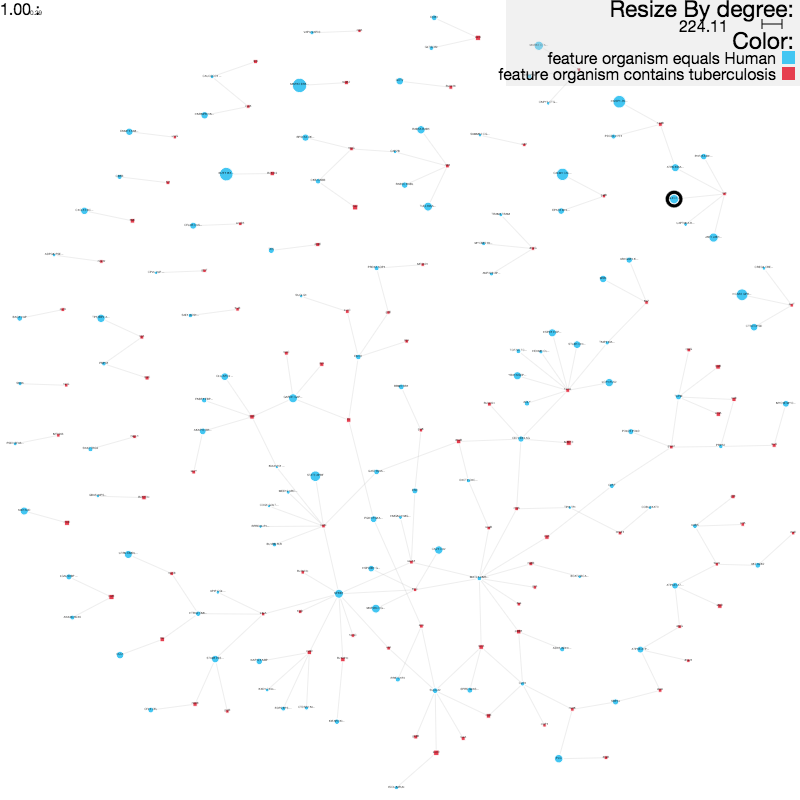
\includegraphics[width=5in]{figures/pinv_human_mtb.png}
\caption[Predicted functional interactions between MTB and Human]{Predicted functional interactions between MTB and Human. Blue circles are human proteins while red squares are from the MTB microorganism.
\label{fig:pinv_human_mtb}}
\end{figure}

\subsection{Research description}
This research is based on the fact that diseases such as tuberculosis are better understood from the relationships between the pathogenous and its host. Some of those relationships can be described as a protein protein interaction, where one protein belongs to the microorganism and the other to the host. Such interaction does not require to be direct (i.e proteins touching each other), and can be what is called a functional interaction, where for instance  the presence of one protein has an effect in the function of another protein. 

Although it is very relevant in the understanding of several biological processes, experimental studies of host-pathogen protein interactions are very scarce, and therefore computational prediction is the available alternative. In this study the authors used the interologs method in order to predict functional interactions between\emph{Mycobacterium tuberculosis} MTB and \emph{Homo Sapiens}. The predicted interactions were filtered, by selecting only the ones differently expressed during infection. The result set was then validated based in the known location of the proteins in the cell, verifying they belong to an area were cross-organism interaction is actually possible. 

The 190 proteins found were further analysed using functional and metabolical pathway knowledge, confirming the potential for some of those proteins to be drug target \cite{RAP2013}. These interactions also illustrate how MTB might acquire nutrients and how it modulates the host response to its advantage.

Figure \ref{fig:pinv_human_mtb} displays the interactions found in this work using PINV.


\subsection{Impact on PINV}

When the first results of this research were presented in a group meeting, the authors expressed the difficulties experienced while exploring the interaction datasets, especially when trying to generate visualisations that will help them to explain their findings. Given our experience with the visualisation projects described in section \ref{section:dasvisual} we took into the challenge of developing a tool that can support research projects that deal with this type of data on the web.

Periodical meetings with the authors of this research help us to define the requirements of PINV and methods to improve the user experience of researchers dealing with protein-protein interaction data. 

The first principle obtained from those meetings was that PINV needed to be more an exploration tool than a graphic generator or an analysis application. And from there comes the decision to have a repository that can be queried in order to extract only the information of interest, instead of loading the whole network in the visualiser, which ultimately ends up in the user requiring to preprocess the data in a separate tool.

\begin{figure}
\centering
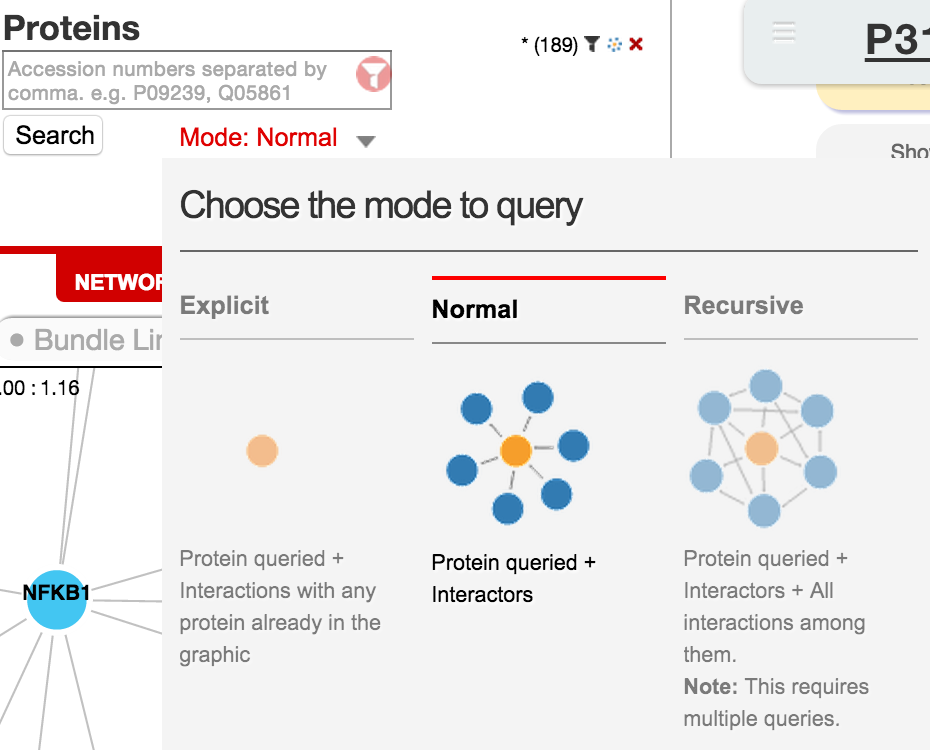
\includegraphics[width=4in]{figures/pinv_modes_query.png}
\caption[Three modes to query by ID in PINV]{Three modes to query by ID in PINV: Explicit, Normal and Recursive
\label{fig:pinv_modes_query}}
\end{figure}

It was with help of our collaborators that we defined the three modes to query by ID (Figure \ref{fig:pinv_modes_query}). PINV's firsts versions only included the normal mode in which a queried protein ID retrieves all the interactions were that protein ID has been reported, but later was pointed out that researchers some times prefer to limit their view to only a subset of proteins, and therefore we developed the explicit mode, and later on the recursive mode was also added as a combination.

Another learnings from these meetings were related to the data itself, on the one hand most of the interaction datasets have similarities, interaction data is  limited to the definition of pairs of biological molecules, information about the origin of the interaction is usually restricted to the method used to discover it. On the other hand, the protein data its heterogeneous, each project select different features to consider, for some, network intrinsic annotations (e.g. degree, closeness, etc.) are the features to consider, while for others, biological features are more relevant (e.g. functional class, cellular location, etc.). 

Based on this we defined that the upload of data to PINV requires two files, one defining the network with all the interactions between proteins and a second file with the annotations of interest for those proteins. A consequence of this open schema for protein data is that PINV widgets, have to adapt to the specificities of each dataset. For example the definition of rules to manipulate the graphic representation consider the features defined for each project, figure \ref{fig:pinv_human_mtb} for instance, uses the degree (i.e. number of connections in the network) of each protein to resize it. Thanks to that, it is easy to identify highly connected proteins, even when the current visualisation is filtering out most of the connections.

One more requirement gathered in this stage was to support direct manipulation of the visualisation; layouts are of great help to start analysing a network, however the researcher often requires to reorganise the network and manually locate some proteins in order to make more evident certain characteristics in the graphic. Therefore, proteins in PINV can be move by dragging them around the graphic, and the simulation forces can be stopped at any time.

\section{Orthologs in 3 Mycobactherium Organisms}\label{sec:orthologs}
\subsection{Research description}
MTP, MLP and MSM

\subsection{Impact on PINV}
multiorganism and filters -TODO: create links with DASty

\section{Shotgun Analysis of Platelets From Dengue Patients}
\label{sec:dengue}
\subsection{Research description}
Real research example

\subsection{Impact on PINV}
Filters and sharing

\section{Human Population Genetics}
\label{sec:pop_genetics}
\subsection{Research description}
Alexia thesis
\subsection{Impact on PINV}
to show the clustering in action!! 


